%% appendix

\section{The Equipartition theorem and the Fluctuation dissapation theorem}

\newpage
\section{Crystal classification, point groups, and Bravais lattices}

\begin{center}
\begin{tabular}{|c|c|c|c|c|}
\hline
\multirow{2}{10em}{Crystal classification} & \multicolumn{2}{|c|}{Point groups} & \multirow{2}{8em}{Bravais lattices} \\ \cline{2-3}
& Hermann-Maugin & Schoenflies & \\
\hline
\multirow{2}{10em}{Triclinic} & 1 & $C_1$ & \multirow{2}{8em}{P} \\
& $\bar{1}$ & $C_i$ &  \\ \hline
\multirow{3}{10em}{Monoclinic} & 2 & $C_2$ & \multirow{3}{8em}{P, C} \\
& $m$ & $C_s$ & \\
& $2/m$ & $C_{2h}$ & \\ \hline
\multirow{3}{10em}{Orthorombic} & 222 & $D_2$ & \multirow{3}{8em}{P, C, I, F} \\
& $mm2$ & $C_{2v}$ & \\
& $mmm$ & $D_{2h}$ & \\ \hline
\multirow{7}{10em}{Tetragonal} & $4$ & $C_4$ & \multirow{7}{8em}{P, I} \\
& $\bar{4}$ & $S_4$ &  \\
& $4/m$ & $C_{4h}$ &  \\
& $422$ & $D_4$ &  \\
& $4mm$ & $C_{4v}$ &  \\
& $\bar{4}2m$ & $D_{2d}$ &  \\
& $4/mmm$ & $D_{4h}$ &  \\ \hline
\multirow{5}{10em}{Trigonal} & $3$ & $C_3$ & \multirow{5}{8em}{R} \\
& $\bar{3}$ & $C_{3i}$ &  \\
& $32$ & $D_3$ &  \\
& $3m$ & $C_{3v}$ &  \\
& $\bar{3}m$ & $D_{3d}$ &  \\ \hline
\multirow{7}{10em}{Hexagonal} & $6$ & $C_6$ & \multirow{5}{8em}{P} \\
& $\bar{6}$ & $C_{3h}$ &  \\
& $6/m$ & $C_{6h}$ & \\
& $622$ & $D_6$ & \\
& $6mm$ & $C_{6v}$ &  \\
& $\bar{6}m2$ & $D_{3h}$ &  \\
& $6/mmm$ & $D_{6h}$ &  \\ \hline
\multirow{5}{10em}{Cubic} & $23$ & $T$ & \multirow{5}{8em}{P, I, F} \\
& $m3$ & $T_h$ & \\
& $432$ & $O$ & \\
& $\bar{4}3m$ & $T_d$ & \\
& $m3m$ & $O_h$ & \\
\hline
\end{tabular}
\end{center}
\textcolor{red}{Crystal Class $\rightarrow$ geometric analogy}
\\
\textcolor{red}{Point groups}
\\
\textcolor{red}{Bravais lattices}
\\
\textcolor{red}{Space groups}

\section{Calibration}
The frequency response measurement shown in (?) records the following transfer function in dB of the following:

\begin{equation}
\alpha(f) = \frac{\mathrm{CH2}(f)}{Source}
\end{equation}

Channel

We also know that the error signal spectra of the loop is probed by $CH2(f)$:


\begin{equation}
\mathrm{CH2}(f) = \frac{\mathrm{S}(f)*signal_V}{(1-\mathrm{OLG}(f))}
\end{equation}

Where $signal_V$ is the uncalibrated voltage output from the mixer, $\mathrm{S}(f)$ is the FSS transfer function, and $\mathrm{OLG}(f)$ is the open loop gain of the PDH system.

And we know $\mathrm{OLG}(f) = \mathrm{S}(f)*\mathrm{A}(f)$ so :

\begin{equation}
\mathrm{signal}_m = \mathrm{CH2}(f)*\mathrm{A}(f) \frac{1-\mathrm{OLG}(f)}{\mathrm{OLG}(f)} \frac{L_\mathrm{cav}}{f_\mathrm{laser}}
\end{equation}

Where $\mathrm{A}*(f)$ is the high voltage amplifier response with the Mephisto 2220 laser PZT response. $L_\mathrm{cav}$ is the sample cavity length, $f_\mathrm{laser}$ is the laser frequency. ($\mathrm{signal}_m$)  is the effective cavity length change from the Pockels effect.

Substitute (1) into (4):

\begin{equation}
\mathrm{signal}_m = \mathrm{Source} * \alpha(f) * \mathrm{A}(f) \frac{1-\mathrm{OLG}(f)}{\mathrm{OLG}(f)} \frac{L_\mathrm{cav}}{f_\mathrm{laser}}
\end{equation}

Measured :
Source, $\alpha (f)$, OLG$(f)$, A$(f)$ and $L_\mathrm{cav}$

\section{Laplace calculator / code}

\section{MACOR assembly}

\begin{figure}[H]
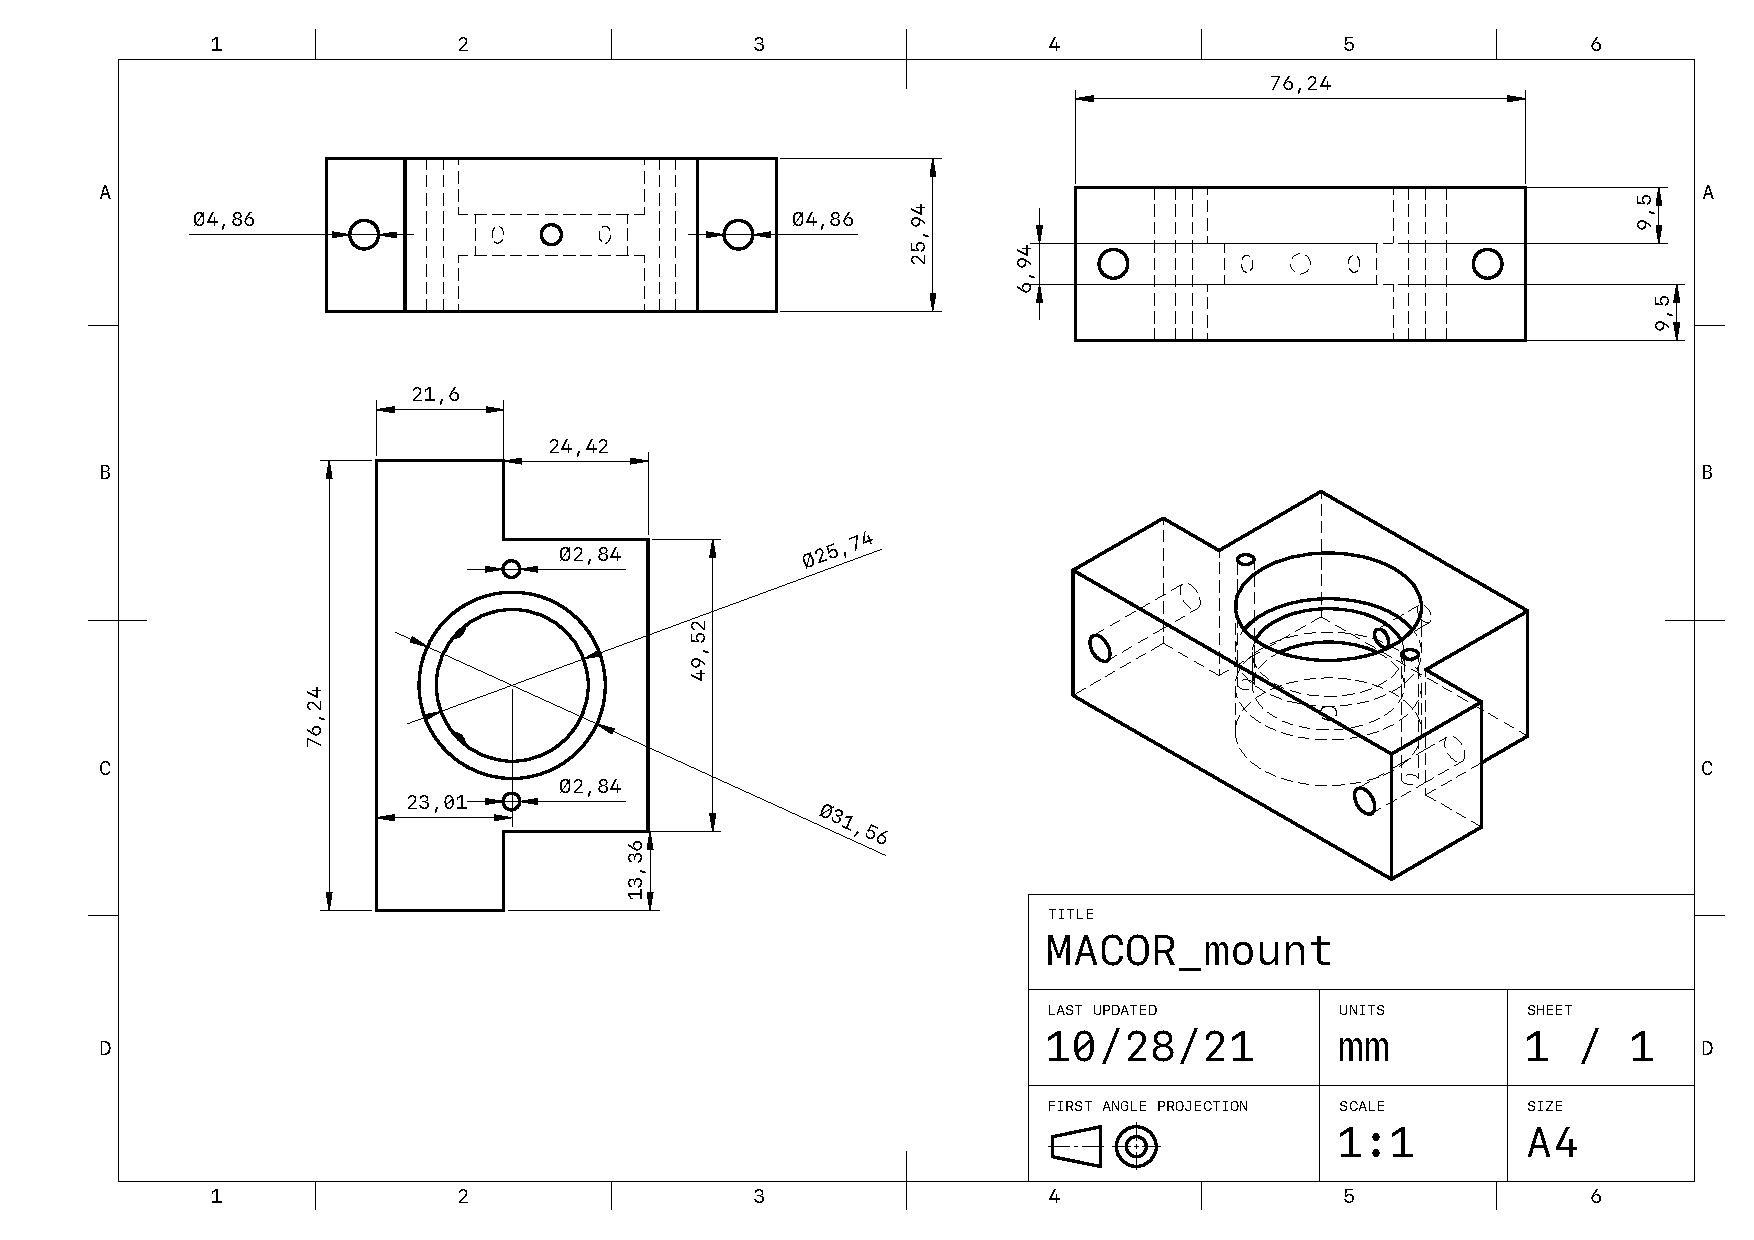
\includegraphics[width=\textwidth]{figs/ALGAAS/MACOR_mount.pdf}
\caption{MACOR mount design constucted in Shapr3D}

\satoshi{First angle projection is used in Europe. In America, third angle projection is used, and I recommend to use it.}

\label{fig:macor_mount_design}
\end{figure}

\section{FSS LTSpice model}

\begin{figure}[H]
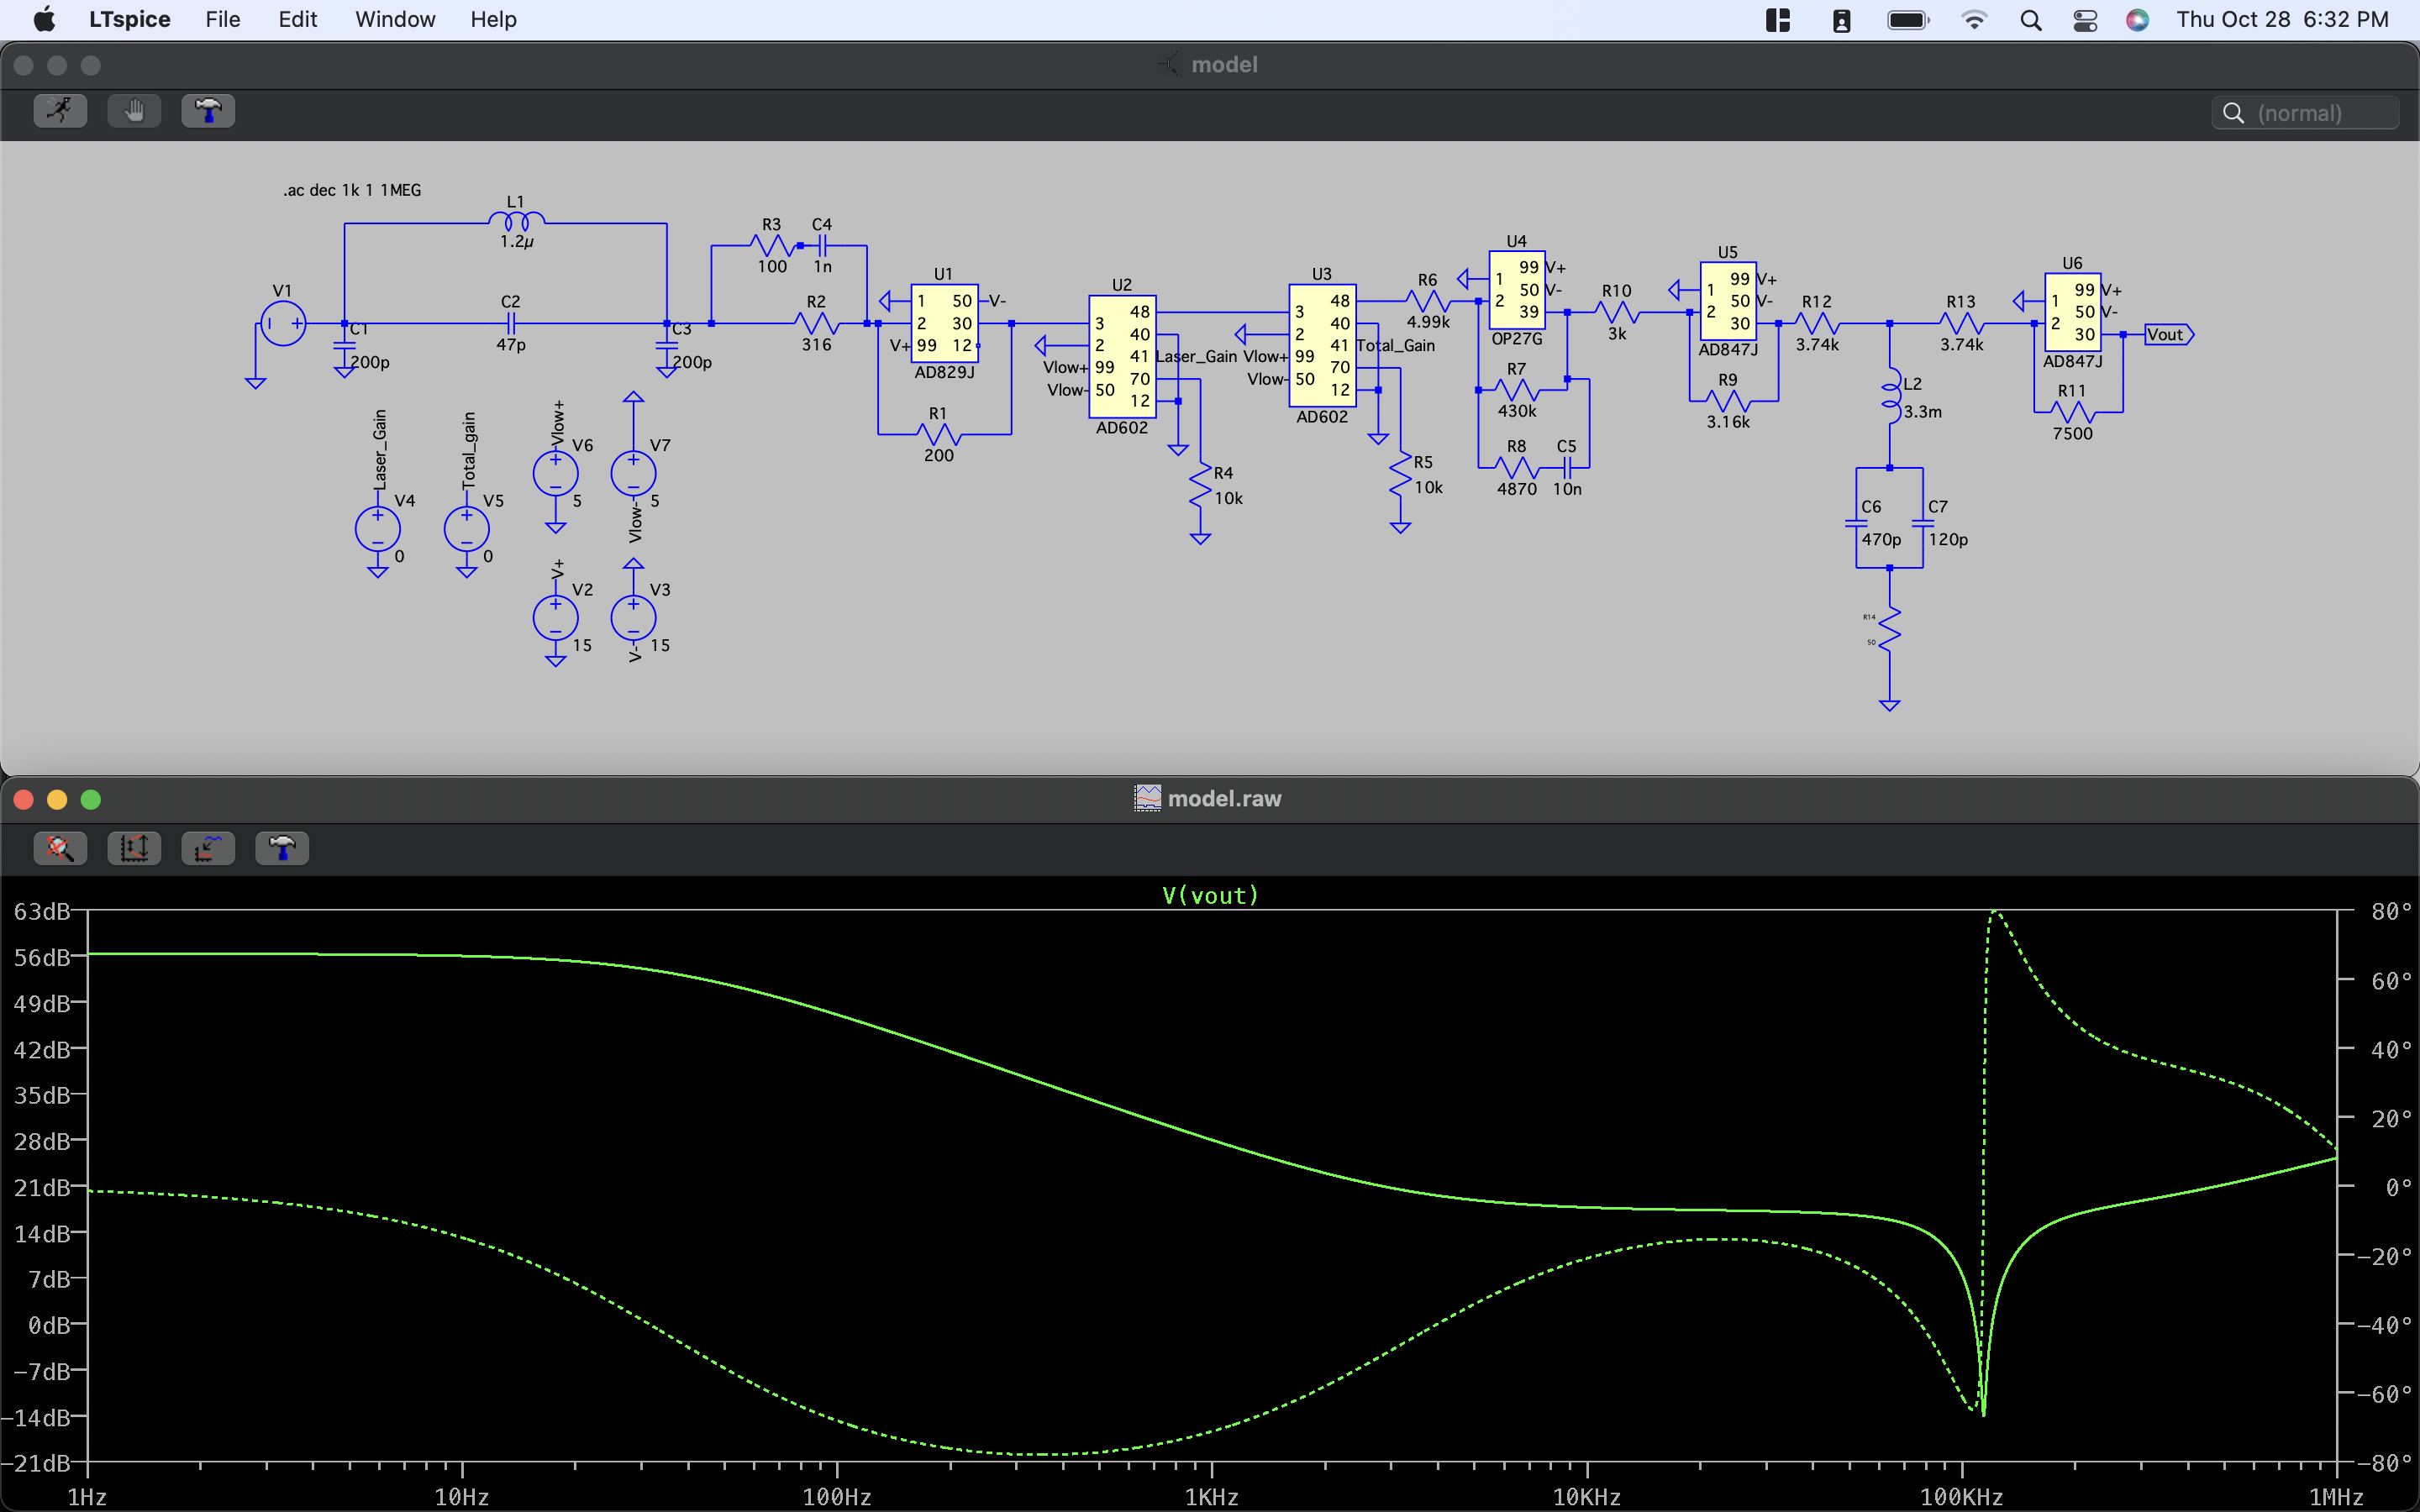
\includegraphics[width=\textwidth]{figs/ALGAAS/spice_FSS_tf.png}
\caption{The FSS transfer function simulated in LTspice}
\label{fig:spiceFSS}
\end{figure}
